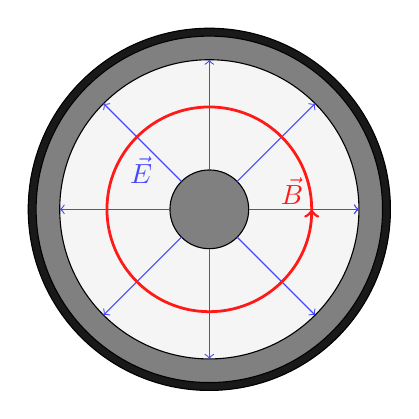
\begin{tikzpicture}
\draw [fill=black!90] (0,0) circle [radius=2.3];
\draw [fill=gray] (0,0) circle [radius=2.2];
% \draw [black] (0,0) circle [radius=2];
\draw [fill=black!4] (0,0) circle [radius=1.9];
\draw [fill=gray] (0,0) circle [radius=0.5];
\foreach \y in {0,45,90,...,360}
{

       \draw [blue!80!white!90, ->] (\y:0.5) -- (\y:1.9);
      %  \pgfmathtruncatemacro{\cur}{\x + 5* \y}
      %  \pgfmathtruncatemacro{\next}{\cur + 1}
      %  \draw (\cur) -- (\next);
}

\draw [red!90,->,line width=1pt] (1.3,0) arc [radius=1.3, start angle=0, end angle= 360];
\node [red!90]at (1.05,0.23) {$\vec{B}$};

\node [blue!80!white!90]at (150:1.0) {$\vec{E}$};

\end{tikzpicture}
